\documentclass{article}
\usepackage{a4wide}
\usepackage{amsthm, amsmath, logicproof, stmaryrd, amssymb, amsfonts}
\usepackage{multicol}
\usepackage{tikz}
\usepackage{macros}
\usepackage{mathrsfs}
\usetikzlibrary{shapes.misc, fit, decorations.pathreplacing,calligraphy,positioning} %for crossing-out arrows and rectangles around nodes
\usepackage{float}
\usepackage{bussproofs}
\usepackage{soul}
\usepackage{todonotes}
\newcommand\rustam[1]{\todo[color=blue!30,size=\small,inline]{Rustam: #1}}
\newcommand\louwe[1]{\todo[color=green!30,size=\small,inline]{Davide: #1}}
\newcommand{\rev}[1]{{\color{blue} #1}}
 %\newcommand{\rev}[1]{{#1}}

\theoremstyle{definition}
\newtheorem{definition}{Definition}[section]
\newtheorem{lemma}{Lemma}
\newtheorem{theorem}{Theorem}
\newtheorem{proposition}{Proposition}


\allowdisplaybreaks

\title{Coalition Strategy Logic}




\date{\today}

\begin{document}
\maketitle

\section{introduction}
\begin{itemize}
    \item An hybrid between SL and CL more powerful than CL
    \item Stackelberger Equilibrium
    \item What we do: axiomatization, model checking, maybe decidability
    
\end{itemize}



\section{Syntax and Semantics}
We define the set $\mathcal{T}$ of \textbf{terms} as the union of the sets $\V$ of variables and $\mathcal{C}$ of constants, we assume that these two sets are, non-empty, at most countable and disjoints.




Given a  positive natural number $n$  and a  countable set $\Ap$  of atomic propositions (that we suppose disjoint from the set of terms), formulae of Coalition Strategy Logic ($\CSL$ for short) are inductively defined by the following grammar: 
$$\varphi := p \mid \neg \varphi \mid \ (\varphi \vee \varphi) \mid \assign{t_1\cdots t_n} \varphi  \mid \forall x \varphi\mid  $$

\noindent where $p$ is any atomic proposition, each of the $t_i$ is a term, and $x$ is a variable. We define the boolean connectives $\land$ and $\to$ and the existential quantifier $\exists$ as usual. 


\begin{definition}
      Given a formula $\varphi$, we define its set of free variables  $\FV(\varphi)  $ by the following cases: 

    \begin{enumerate}
        
        \item If $\varphi\in \Ap$ then $\FV(\varphi)=\emptyset$; 
        \item If $\varphi=\neg \varphi_1$ then $\FV(\varphi)=\FV(\varphi_1)$; 
        \item If $\varphi=\varphi_1 \vee \varphi_2$ then $\FV(\varphi)=\FV(\varphi_1)\cup \FV(\varphi_2)$; 
        \item if $\varphi=\assign{t_1\cdots t_n }\varphi_1$ then 
       $\FV(\varphi)=\FV(\varphi_1)\cup \set{t_i \mid t_i\in \V} $
        
     \item if $\varphi= \forall x \varphi_1$ then $\FV(\varphi)=\FV(\varphi_1)\setminus \set{x}$:
       
        
    \end{enumerate}

    \noindent A formula $\varphi$ such that $\FV(\varphi)=\emptyset$ is called a \textbf{sentence}.
\end{definition}



\begin{definition}
    A Kripke Frame is a tuple $\mathcal{F}=\tuple{\Sigma,S,R}$ where, $\Sigma$ is a non-empty countable alphabet, $S$ is a non-empty countable set of states  (that we suppose disjoint from $\Sigma$) and  $R\subseteq S\times \Sigma \times S$ is a ternary relation, dubbed transition relation. We say that $\mathcal{F}$ is: 
    \begin{itemize}
        \item[] \textbf{serial} whenever $R$ is, that is: for every $x\in S$ for every $a\in \Sigma$ there is a  $y\in S$ such that $\tuple{x,a,y}\in R$ ; 
        \item[]\textbf{functional} whenever $R$ is, hat is : for every $x,y,z\in S$ and for every $a\in \Sigma$ if $\tuple{x,a,y}\in R$ and $\tuple{x,a,z}\in R$ then $y=z$. 
      \end{itemize}


\end{definition}


\begin{definition}
    A game frame is a tuple $\mathcal{G}=\tuple{n,\Ac, \mathcal{D}, S,R }$ where: 
    \begin{itemize}
        \item $n$ is a positive natural number; 
        \item $\Ac$ is a countable set of actions; 
        \item $\mathcal{D}$ is the set of tuples of elements of $\Ac$ of length $n$ (elements of this set will be called decisions); 
        \item $S$ is a countable  set of states; 
        \item $R\subseteq S \times \mathcal{D}\times S$ is a ternary relation; 
        
    \end{itemize}
    
    Such that the triple $\tuple{\mathcal{D}, S, R}$ is a serial and functional Kripke Frame. A concurrent game structure is a pair $\mathfrak{G}=\tuple{\mathcal{G},\mathcal{V}}$ where $\G$ is a Game Frame and $\mathcal{V}: \Ap \to \mathcal{P}(S)$ is a function sending each atomic proposition to a subset of the set of states of $\mathcal{G}$. 
\end{definition}



%\begin{definition}
 %   Given a CGS $\G$, an assignment over $\G$ is a map 
  %   $\sigma : \V  \to \Ac$ sending each variable to an action. If $\sigma$ is an assignment, $v\in \V $ and $a\in \Ac$, we let $\sigma[a/v]$ denote the assignment $\sigma'$ such that $\sigma'(v')=\sigma(v')$ when $v'\neq v$ and $\sigma'(v)=a$.

    
     
 
%\end{definition}




\begin{definition}
    Given a CGS $\G$, the language  $\mathfrak{L}(\G)$ of $\G$ is the language in which the set of constants contains a constant symbol $\overline{a}$ for any action $a\in \Ac$ and nothing else. 
 \end{definition}







\begin{definition}
Given a CGS $\G$ a state $s$ of $\G$, and a closed  formula $\varphi$ constructed over $\mathfrak{L}(\G)$, the  satisfaction relation $\G,s\models \varphi$ is inductively defined on the structure of $\varphi$ as follows: 
    \begin{itemize}
    \item $\G,s\models p$ iff $s\in \mathcal{V}(p)$; 
    \item $\G,s \models \neg \psi$ iff it is not the case that $\G,s \models \psi$ (denoted $\G,s\not\models \psi)$; 
    \item $\G,s\models \theta \vee\psi $ iff $\G,s \models \theta$ or $\G,s \models \psi$;
    \item $\G,s \models \assign{    \overline{a_1}\cdots \overline{a_n}} \psi $ iff there is $s'$ such that $\tuple{s, {a_1}\cdots {a_n},s'}\in R$ and $\G,s'\models  \psi $ 
    
    \item $\G,s,\sigma \models \exists x \psi$ iff for every   $a \in \Ac$ we have that $\G,s \models \psi[\overline{a}/x]$.
    
\end{itemize}


\noindent where $\psi[\overline{a}/x]$ denotes the result of substituting every occurrence of the variable $x$ with the constant $\overline{a}$ in $\psi$.  
    
\end{definition}


We can show the following easy proposition. 

\begin{proposition}
    Let $\G$ be a game model, $s$ any of its states and $\varphi$ a formula of the form $\assign{\overline{a_1}\cdots \overline{a_n}} \psi$, we have that $\G,s \models \varphi$ if and only if, for every state $y$ of $\G$ if $\tuple{x,a_1,\,\ldots, a_n,y}\in R$ then $\G,y\models \psi$. 
    
     \end{proposition}
   \begin{proof}
       The left-to-right direction is granted because of seriality, while the converse direction is granted because of  totality. 
   \end{proof}

   In virtue of the above proposition, we will freely switch between the two definitions of satisfaction for formulas of the form  $\assign{\overline{a_1}\cdots \overline{a_n}} \psi$. 



   

\section{Relation to Other Formalisms}
In order to appreciate the richness of $\CSL$, we compare the logic to other related logics of strategic ability. In our comparison we will use two salient features of $\CSL$. First, the logic allows for \textit{arbitrary quantification prefixes for agents' strategies}. This includes using the same strategy variable for different agents to capture \textit{strategy sharing}. The second special feature of $\CSL$ is the presence of \textit{explicit action labels} in its syntax.

These two features on their own are not unique in the landscape of logics for strategic reasoning. Thus, arbitrary quantification prefixes is a hallmark feature of the whole family of \textit{strategy logics} (see, e.g., \cite{mogavero10,belardinelli19}), to which $\CSL$ belongs. Indeed, $\CSL$ can be considered as a variation of the next-time fragment of \textit{strategy logic with simple goals} ($\mathsf{SL[SG]}$) \cite{belardinelli19}, which, in turn, is an extension of $\mathsf{ATL}$ \cite{alur02} with arbitrary quantification prefixes for agents' strategies. The idea to refer to action in the language has also been explored, with, perhaps, a prime example being $\mathsf{ATL}$ \textit{with explicit strategies} ($\mathsf{ATLES}$) \cite{walther07}. Another example of a logic with explicit actions is \textit{action logic} ($\mathsf{AL}$) \cite{borgo07}, which we will look at closer later in this section.

Even though both of the main features of $\CSL$ have been somewhat explored in the literature, to the best of our knowledge, $\CSL$ is the first logic for strategic reasoning that combines \textit{both} of them. To further demonstrate the unique position our logic has in the landscape of related logics, we compare it some coalition logics explored in literature. 

%It is easy to show that $\CSL$ and $\mathsf{ATLES}$ are, expressivity-wise, incomparable. Indeed, in the former we can exploit arbitrary quantification prefix, and in the latter we have additional temporal expressivity. 

 %Moreover, $\CSL$ allows for actions of agents to be explicitly referenced in the logic language. These two features combined, i.e. arbitrary quantification prefixes and explicit action labels, make $\CSL$ quite unique in the landscape of the logics for strategic reasoning. 

 \paragraph{Coalition logic} The original \textit{coalition logic} ($\mathsf{CL}$) \cite{pauly02}, similarly to $\mathsf{ATL}$, allows only single alternation of quantifiers in coalitional modalities. Moreover, this quantification is implicit. Thus, $\mathsf{CL}$ extends the language of propositional logic with constructs $\langle \! \langle C \rangle \! \rangle \varphi$ that mean `there is a strategy for coalition $C$ to achieve $\varphi$ in the next step (whatever agents outside of the coalition do at the same time)'. 
 
 To introduce the semantics of $\mathsf{CL}$, we will denote the choice of actions by coalition $C \subseteq Agt$ as $\sigma_C$, and denote $Agt \setminus C$ as $\overline{C}$. Finally, $\sigma_C \cup \sigma_{\overline{C}} \in \mathcal{D}$ is a decision. The semantics of $\langle \! \langle C \rangle \! \rangle \varphi$ for a given CGS $\G$ is then defined as 
  \begin{alignat*}{3}
        &\G,s \models \langle \! \langle C \rangle \! \rangle \varphi && \text{ iff } && \exists \sigma_C, \forall \sigma_{\overline{C}} : \G,t \models \varphi \text{ with } t \in S \text{ such that } \langle s, \sigma_C \cup \sigma_{\overline{C}}, t \rangle \in R.   
\end{alignat*}     
 
The translation from formulas $\mathsf{CL}$ to formulas of $\CSL$ can be done recursively using the following schema for coalitional modalities: 
$tr(\langle \! \langle C \rangle \! \rangle \varphi) \to \exists \vec x \forall \vec y \assign{\vec x, \vec y} tr(\varphi)$, 
where variables $\vec x$ quantify over actions of $C$, and $\vec y$ quantify over actions of $Agt \setminus C$. 

At the same time, one cannot refer to particular strategies in $\mathsf{CL}$ formulas, as well as express sharing strategies between agents. We can exploit either of these feature to show that $\CSL$ is strictly more expressive than $\mathsf{CL}$. 
Indeed, consider a $\CSL$ formula $\exists x \assign{x, x} \lnot p$ meaning that there is an action that \textit{both} agents 1 and 2 can use to reach a $p$-state. We can construct two concurrent game structures that are indistinguishable by any $\mathsf{CL}$ formulas. At the same time,   $\exists x \assign{x, x} \lnot p$ will hold in one structure and false in another. 

Consider two structures depicted in Figure \ref{fig::exampleCGM}. 

\begin{figure}[h!]
\centering
\scalebox{1}{
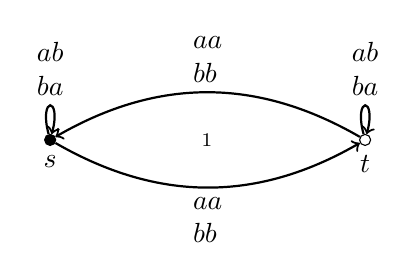
\begin{tikzpicture}
\node(-1) at (2,0) {$\G_1$};
\node[circle,draw=black, minimum size=4pt,inner sep=0pt, fill = black, label=below:{$s$}](1) at (0,0) {};
\node[circle,draw=black, minimum size=4pt,inner sep=0pt, , label=below:{$t$}](2) at (4,0) {};

\draw [->,thick](1) to [loop above] node[above, align=left] {$ab$\\$ba$} (1);
\draw [->,thick](1) to [bend right] node[below,align=left] {$aa$\\$bb$} (2);
\draw [->,thick] (2) to [bend right] node[above,align=left] {$aa$\\$bb$} (1);
\draw [->,thick] (2) to [loop above] node[above,align=left] {$ab$\\$ba$} (2);
\end{tikzpicture}
\hspace{10mm}
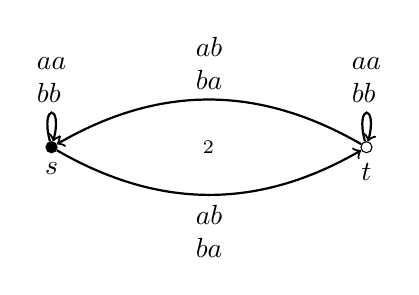
\begin{tikzpicture}
\node(-1) at (2,0) {$\G_2$};
\node[circle,draw=black, minimum size=4pt,inner sep=0pt, fill = black, label=below:{$s$}](1) at (0,0) {};
\node[circle,draw=black, minimum size=4pt,inner sep=0pt, , label=below:{$t$}](2) at (4,0) {};

\draw [->,thick] (1) to [loop above] node[above, align=left] {$aa$\\$bb$} (1);
\draw [->,thick](1) to [bend right] node[below,align=left] {$ab$\\$ba$} (2);
\draw [->,thick] (2) to [bend right] node[above,align=left] {$ab$\\$ba$} (1);
\draw [->,thick] (2) to [loop above] node[above,align=left] {$aa$\\$bb$} (2);
\end{tikzpicture}
}
\caption{CGSs $\G_1$ and $\G_2$ for two agents and two actions. Propositional variable $p$ is true in black states.}
\label{fig::exampleCGM}
\end{figure} 
It is easy to see that $\G_1,s$ and $\G_2,s$ cannot be distinguished by any $\mathsf{CL}$ formula. Indeed, both structures agree on valuation of propositional variable $p$ in corresponding states. Moreover, none of the agents, 1 and 2, can on their own force a transition from state $s$ to state $t$. At the same time, the grand coalition $\{1,2\}$ can force the transition in both structures. Now, we can verify that $\G_1,s \models \exists x \assign{x, x} \lnot p$ and $\G_2,s \not \models \exists x \assign{x, x} \lnot p$. For the case of  $\G_1,s \models \exists x \assign{x, x} \lnot p$, it is enough to assign action $a$ to $x$ to have $\G_1,s \models \assign{a, a} \lnot p$. To make $\G_2,s \not \models \exists x \assign{x, x} \lnot p$ hold, one needs to provide an action that once being executed by both agents will force the transition to state $t$. It is easy to see that there is no such an action in $\G_2,s$.

Having the translation from $\mathsf{CL}$ to $\CSL$ on the one hand, and the indistinguishability result on the other, we hence conclude that $\CSL$ is \textit{strictly more expressive} than $\mathsf{CL}$.

\paragraph{Conditional strategic reasoning and socially friendly coalition logic} With the expressive power of $\CSL$ we can go much further than the classic $\mathsf{CL}$. In particular, we can express in our logic such interesting coalition logics like \textit{logic for conditional strategic reasoning} \cite{goranko22}, \textit{socially friendly coalition logic} \cite{goranko18}, and \textit{group protecting coalition logic}  \cite{goranko18}. 

Presenting semantics of the aforementioned logic is beyond the scope of this paper. However, we would like to point out that all of the logics can be captured by \textit{basic strategy logic} ($\mathsf{BSL}$) \cite{goranko23}, which is a variant of $\mathsf{SL}$ where each agent has her own associated strategy variable. Differently from $\CSL$, $\BSL$ allows for all standard temporal modalities like `ne\textsf{X}t', `\textsf{U}ntil' and `\textsf{G}lobally (or Forever)'. At the same time, $\BSL$ does not allow for variable sharing and does not explicitly refer to actions or strategies. Moreover, it is conjectured \cite{goranko23} that $\BSL$ does not have a recursive axiomatisation, while $\CSL$ has a finitary sound and complete axiomatisation (see Section \textbf{???}).

Translations of all coalition logics introduced in this paragraph into formulas of $\mathsf{BSL}$ is presented in \cite{goranko23}. The translation does not employ any temporal features of $\mathsf{BSL}$ apart from `ne\textsf{X}t', and thus the same translation also works for $\CSL$. 



\paragraph{Coalition action logic} 

A perhaps the most relevant to $\CSL$ coalition logic in the literature is \textit{action logic} ($\mathsf{AL}$) \cite{borgo07}, which is a fragment of \textit{multi-agent PDL with quantificaiton} ($\mathsf{mPDLQ}$) \cite{borgo05}. $\mathsf{AL}$ extends the language of propositional logic with so-called \textit{modality markers}, which are, essentially, quantification prefixes $Q_1 x_1, ..., Q_n x_n$ of size $|Agt| = n$ and where $Q_i \in \{\forall, \exists\}$. Then, formula $[Q_1 x_1, ..., Q_n x_n]\varphi$ holds in a CGS, if and only if all outcomes resulting in assigning actions to agents based on the quantification prefix lead to $\varphi$-states. It is easy to see that formulas $[Q_1 x_1, ..., Q_n x_n]\varphi$ with modality markers can be trivially translated into formulas of $\CSL$ of the form $Q_1 x_1, .., Q_n x_n \assign{x_1, ..., x_n} \varphi$. Moreover, $\mathsf{AL}$ does not allow for sharing strategies (while $\CSL$ does), i.e. all $x_1, ..., x_n$ in the modality marker are unique. Finally, to the best of our knowledge, there is no axiomatisation of  $\mathsf{AL}$.


\section{Proof theory}


The axiom system $\CSL$ consist of the following axiom schemata and rules, where $\vec{t}=t_1,\ldots,t_n$ for $n\geq 1$
$$
\begin{array}{c
%@{\qquad}
l}

    \mathsf{IPL}  & \text{Every propositional tautology}  
  \\
  \\
     \mathsf{K} & ( \assign{\vec{t}} \varphi \land \assign{\vec{t}}\psi) \iff \assign{\vec{t}}(\varphi \land \psi )
   \\
   \\
   \mathsf{\mathsf{N} } & \neg \assign{\Vec{t}}\varphi \iff \assign{\vec{t }}\neg \varphi 

   \\
   \\
   \mathsf{E} & \forall x \varphi \to \varphi[t/x]
\\
\\
\mathsf{B} & \forall x \assign{\vec t} \varphi \imp \assign{\vec t} \forall x \varphi \qquad % x\neq t_i \text{ for all $i\leq n$} 
\end{array}$$

\begin{tabular}{p{0.33\textwidth} p{0.33\textwidth} p{0.33\textwidth}}

   \begin{prooftree}
       \AxiomC{$\varphi$}\LeftLabel{$\mathsf{MP}$}
       \AxiomC{$\varphi \to \psi$}
       \BinaryInfC{$\psi$}
   \end{prooftree} 
   &  
  \begin{prooftree}
       \AxiomC{$\varphi$}\LeftLabel{$\mathsf{Nec}$}
         \UnaryInfC{$\assign{\vec t }\varphi $}
   \end{prooftree} 
   
     &  \begin{prooftree}
       \AxiomC{$\varphi\to \psi $}\RightLabel{$x\notin \FV(\varphi  )$}\LeftLabel{$\mathsf{Gen}$}
        \UnaryInfC{$\varphi\to \forall x \psi$}
   \end{prooftree} 

     
\end{tabular}



\noindent An axiomatic derivation $\pi$ is a finite sequence of formulae $\varphi_1,\ldots, \varphi_m$ where for each $i\leq m$:  either $\varphi_i$ is an instance of one of the rule schemata of $\CSL$, or it is obtained by some preceding formulae in the sequence using the rule $\mathsf{MP}$, the rule $\mathsf{Nec}$, or the rule $\mathsf{Gen}$
We write $\vdash_\CSL \varphi$ and we say that  $\varphi$ is \emph{CSL derivable} (or simply derivable)  iff there is a derivation $\pi$ whose last element is $\varphi$. Given a set of formulae $X$, we write $X \vdash_\CSL \varphi$ iff there is a finite subset $Y $ of $X$ such that $\vdash_\CSL \bigwedge Y \imp \varphi$. 

\begin{definition}
Let $X$ be a set of $\CSL$ formulas. We say that: 
\begin{itemize}
    \item $X$ is \emph{consistent} iff $X\not\vdash_\CSL \bot$
    \item $X$ is maximally consistent iff it is consistent and there is no other consistent set of formulas that strictly includes $X$; 
\item $X$ has the Henkin property iff for any formula of the form $\exists x \varphi$, if $\exists x \varphi \in X$ then there is a constant $a$ such that $\exists x \varphi \imp \varphi [a/x]\in X$.  

    \end{itemize}

  
\end{definition}

%The $\forall$-property is a standard way in quantified modal logics to tackle non-compactness. Indeed, consider the set $\Delta = \{\lnot \forall x \varphi, \varphi[a_1/x], \varphi[a_2/x]...\}$. It is easy to see that each finite subset of $\Delta$ is satisfiable, while the whole $\Delta$ is not. Now, if some set $\Gamma$ is maximal, consistent, and has the $\forall$-property, then every instance of $\forall x \varphi \not \in \Gamma$ will be witness by some $\varphi[a/x] \not \in \Gamma$.




\begin{definition}
    Let $X$ be a set of sentences constructed over a set of constants $Ac$. Let $Ac^\star$ be the set of constants obtained by adding to $Ac$ a constant $a_{\varphi}$ for each sentence of the form $\exists x \varphi$. Then the set $X^\star$ is the set of formulas constructed over $Ac^\star$  such that $X^\star = X \cup \set{\psi \mid \psi = \exists x \varphi \imp \varphi[a_\varphi /x]}$ 
\end{definition}


The proof of the following lemmata are completely standard. 
\begin{lemma}
    If $X$ is a consistent set of sentences, then $X^\star$ has the Henkin property and for any formula $\varphi$ that is constructed over $Ac$ we have that $X^\star \vdash_\CSL \varphi$ iff $X\vdash_\CSL \varphi$, thus $X^\star$ is consistent. 
\end{lemma}

\begin{lemma}
\label{lemma:lindy}
    Every consistent set of sentences having the Henkin property can be extended into a maximally consistent set of sentences having the Henkin property. 
\end{lemma}



%\begin{lemma}
 %   Let $X$ be any consistent set of formulas that are constructed over a set $Ac$ of actions. There is a set $Y$ of formulas such that 
%\end{lemma}

%\begin{lemma}
%Let $\Gamma$ be a consistent set of formulas of $\CSL$. Then there is a consistent set $\Delta$ of formulas of $\CSL^+$ such that $\Delta$ has the $\forall$-property and $\Gamma \subseteq \Delta$, and where $\CSL^+$ is the extension of $\CSL$ with a new countably infinite set of variables. 
%\end{lemma}

%Hi!

%Next, we need to show that if some formula $\assign{\Vec{t}} \varphi \not \in \Gamma$, then there is a witness set $\Delta$ such that $\lnot \varphi \in \Delta$.

%begin{lemma}
%Let $\Gamma$ be an MCS$^\forall$, and $\assign{\Vec{t}} \varphi \not \in \Gamma$, where $\Vec{t}$ contains only constants. Then there exists an MCS$^\forall$ $\Delta$ over $\CSL^+$ such that $\assign{\Vec{t}} \Gamma \cup \{\lnot \varphi\} \subseteq \Delta$.
%\end{lemma}

%\begin{proof}
    
%\end{proof}

\rustam{There is some mismatch in notation with the canonincal model in the definiton and later in proofs}

\begin{definition}[Canonical Model]
\label{def:can_model}

The canonical model is the tuple $\G^C=\tuple{Ac^C,S^C,\mathcal{D}^C,R^C,    \mathcal{V}^C}$ where: 

\begin{itemize}
    \item each member of $S^C$ is a maximally consistent set of sentences having the Henkin property. 
    \item the set $Ac^C$ of actions is equal to the set  $\set{a \mid  a\text{ occurs in } \varphi \in X \text{ for some } X\in S^C}$
    \item $\mathcal{D}^C$ is ${Ac^C}^n $
    \item $\tuple{X,a_1,\ldots , a_n, Y}\in R^C$ iff for every formula $\assign{a_1,\ldots, a_n}\varphi\in X$ the formula $\varphi\in Y$
    \item finally, $X \in \mathcal{V}^C(p)$ iff $p\in X$. 
\end{itemize}
    
\end{definition}

\begin{proposition}
    The canonical model $\G^C$ is a game model. 
\end{proposition}
\begin{proof}
    \rev{It is enough to note that} 
    each member of $S^C$ contains the formula $\neg \assign{a_1,\ldots,a_n}\varphi \iff \assign{a_1,\ldots, a_n} \neg \varphi$ for each $a_i\in Ac^S$.  This forces the relation $R^S$ to be serial and functional.  
\end{proof}

We state another lemma whose proof is completely standard. 

\begin{lemma}
\label{lemma:diamond}
Let $\vec a= a_1,\ldots a_n$: 
if the set of sentences $\set{\neg \assign{\vec a}\varphi, \assign{\vec a} \psi_1, \assign{\vec a} \psi_2,\ldots }$ is consistent, so is the set $\set{\neg \varphi, \psi_1, \psi_2 \ldots }$
    \end{lemma}

    \rustam{Maybe it would be nice to give the sketch of the above lemma to demonstrate why we need the barcan formula}

We conclude by stating the canonical model Lemma. 

\begin{lemma}[Truth Lemma]
For any state $X$ of the canonical model $\G^C$ and for any formula $\varphi$, we have that $\varphi \in X$ iff $\G^C, X \models \varphi$. 
\end{lemma}
\begin{proof}
    The proof is by induction on $\varphi$: the base case in which $\varphi$ is an atomic proposition immediately follows by the definition of $\mathcal{V}^C$. The cases in which $\varphi$ is a Boolean formula immediately follows by induction hypothesis and by the properties of maximal consistent sets.

 \begin{itemize}
     \item if $\varphi$ is $\assign{\vec{a}} \psi$
    \begin{itemize}
        \item[] Suppose that  $\varphi \in X$ and let $Y$ be an arbitrary member of $S^C$ such that $\tuple{X,\vec{a}, Y}\in R^C$. By the definition of $R^C$ we must have that $\psi \in Y$ and by induction hypothesis  $\G^C, Y \models \psi$ and since $Y$ is arbitrary we conclude that $\G^c, X \models \varphi$.  
        \item[] Assume that $\varphi \notin X$, Since $X$ is maximally consistent, we have that $\neg \assign{\vec a} \psi \in X$. Let $\set{\assign{\vec a} \psi_1, \assign{\vec a}\psi_2,\ldots }$ the set of all members of $X$ starting with $\assign{\vec a}$. The  set $\set{\neg \assign{\vec a}\psi, \assign{\vec a} \psi_1, \assign{\vec a}\psi_2,\ldots }$ is contained in $X$ and it thus consistent. By Lemma \ref{lemma:diamond} also the set $\set{\neg \psi, \psi_1, \psi_2, \ldots}$ is consistent and it can be thus extended to a maximal consistent set $Z$ having the Henkin property.  Furthermore, by definition of $R^C$ we have that $\tuple{X, \vec a , Z}\in R^C$. Since $\neg \psi\in Z$ we deduce that $\psi \notin Z$ and thus, by induction hypothesis, $\G^C, Z \not\models \psi$ but this means that $G^C, X \not \models \assign{ \vec a}\psi $.

    \end{itemize} 

    \item if $\varphi$ is $\forall x \psi $

    \begin{itemize}
        \item[] Suppose $\varphi\in X$, since $X$ is maximally consistent we have that $X\vdash_\CSL \varphi$ and by axiom $\mathsf{E}$ and $\mathsf{MP}$ we obtain that $X\vdash_\CSL \psi[a / x]$ for all $a\in Ac$, and thus $\psi[a/x]\in X$ for each $a\in Ac^S$. By induction hypothesis $\G^C,x \models \psi[a/x]$ for each action $a$. We conclude that $\G^C, X \models \varphi$. 
        \item[] Conversely, assume that $\G^C, X \models \varphi$. By the truth definition and induction hypothesis, we obtain that $\psi[a/x]\in X$ for all $a\in Ac^C$. 
        \rev{It is not super clear that we gonna have $\exists x \lnot \psi \in X$ to state the following. Shouldn't we prove this case using the contrapositive? Like $\varphi \not \in X$, then $\exists x \lnot \psi \in X$, and then the Henkin property?}
        Consider an action $b\in Ac^C$ such that $\exists x \neg \psi \imp \psi [b/x]\in X$. 
        We obtain that $X\vdash_\CSL \exists x \neg \psi \imp \psi [b/x] $  and also that $X \vdash \psi [b/x]$ thus, by classical reasoning, that $X\vdash_\CSL \neg \exists x \neg \psi$. Since $\neg \exists x \neg \psi \equiv \forall x \psi $ we can conclude \rev{that $\forall x \psi \in X$}.   
    \end{itemize}

\end{itemize}\end{proof}
    

%    \textit{Case} $\varphi=\assign{\vec a} \psi$.  Assume that $\assign{\vec a} \psi \in X$, and that there is some $Y$ such that $\tuple{X,a_1,\ldots , a_n, Y}\in R^C$. By the construction of the canonical model, the latter is equivalent to the fact that $\psi \in Y$, which, in turn, is equivalent to $\G^C, Y \models \psi$ by the induction hypothesis. Finally, $\tuple{X,a_1,\ldots , a_n, Y}\in R^C$ and $\G^C, Y \models \psi$ is equivalent, by the definition of the semantics, to $\G^C, X \models \assign{\vec a} \psi$. 
%$$    \textit{Case} $\varphi=\forall x \psi$. \textit{From left to right.} Assume that $\forall x \psi \in X$, and let $\sigma^\prime$ be an arbitrary assignment  WAIt. Let me do it, i have an hour right now
 %   alright! noice 
    %I'll go and eat something then!
    
    %When $\varphi=\assign{\vec a} \psi$


    


    


\bibliographystyle{plain}
\bibliography{cslref}

\end{document}